\section{Testing}
\headerblock{
  \headerquote{The return on investment from random testing is good. Our rough
  estimate—including faculty, staff, and student salaries, machines
  purchased, and university overhead—is that each of the more than
  325 bugs we reported cost less than \$1,000 to find.}{Yang, Chen, Eide, and Regehr~\cite{yang2011finding}}
}
\label{sec:testing}

\subsection{Motivating Examples}
\label{ssec:motivating-examples}

Programs written in distributed stream processing frameworks exhibit implicit parallelism, which can lead to subtle bugs. Programs in such frameworks are usually written as \emph{dataflow graphs}, where the edges are data streams and the nodes are streaming operators or transformations.
Common operators include stateless transformations (\emph{map}), and operations that group events based on the value of some field (\emph{key-by}).
For example, suppose that we have a single input stream which contains information about rides of a taxi service: each input event $(\texttt{id}, \texttt{pos}, \texttt{meta})$ consists of a taxi identifier, the taxi position, and some metadata. In the first stage, we want to discard the metadata component (\emph{map}) and partition the data by taxi ID (\emph{key-by}). In the second stage, we want to aggregate this data to report the total distance traveled by each taxi. Notice that the second stage is order-dependent (events for each taxi need to arrive in order), so it is important that the first stage does not disrupt the ordering of events for a particular taxi ID.

\begin{figure}[tb]
\centering
\begin{tikzpicture}[node distance=0.5cm,every node/.style={font=\footnotesize}]
\node[source] (in) {input};
\node[operator, right=of in] (op1) {\texttt{project(taxiID, position)}};
\node[operator, right=of op1] (op2) {\texttt{keyBy(taxiID)}};
\node[sink, right=of op2] (out) {output};
\node[right=of out,minimum width=2cm] (label) {\textbf{\emph{(Incorrect)}}};

\draw[dataflowedge] (in) -- (op1);
\draw[dataflowedge] (op1) -- (op2);
\draw[dataflowedge] (op2) -- (out);
\end{tikzpicture}

\smallskip

\begin{tikzpicture}[node distance=0.5cm,every node/.style={font=\footnotesize}]
\node[source] (in) {input};
\node[operator, right=of in] (op1) {\texttt{keyBy(taxiID)}};
\node[operator, right=of op1] (op2) {\texttt{project(taxiID, position)}};
\node[sink, right=of op2] (out) {output};
\node[right=of out,minimum width=2cm] (label) {\textbf{\emph{(Correct)}}};

\draw[dataflowedge] (in) -- (op1);
\draw[dataflowedge] (op1) -- (op2);
\draw[dataflowedge] (op2) -- (out);
\end{tikzpicture}

\caption{A subtle consequence of implicit parallelism
over an input stream containing taxi location data.
}
\label{ex:overview-simple}
\end{figure}

To make a program for the first stage of this computation in a distributed stream processing framework such as Flink or Storm, we need to build a dataflow graph representing a sequence of transformations on data streams. A first (natural) attempt to write the program is given in \cref{ex:overview-simple} (top). Here, the \texttt{project} node projects the data to only the fields we are interested in; in this case, \texttt{taxiID} and \texttt{position}. And \texttt{keyBy} (also known as ``group by'' in SQL-like languages, or the concept of a ``stream grouping'' in Storm) partitions the data stream into substreams by \texttt{taxiID}.
Although written as an operator, here \texttt{keyBy} can be thought of as modifying the stream to give it a certain property (namely, if it is parallelized, streams should be grouped by the given key).

The first attempt is incorrect, however, because it fails to preserve
the order of data for a particular key (taxi ID), which is required
for the second stage of the computation. The problem is that dataflow
graph operators are implicitly parallelized---here, the stateless map
\texttt{project} is internally replicated into several copies, and the
events of the input stream are divided among the copies.
Because input events of the same key may get split across substreams,
when the operator \texttt{keyBy} reassigns each item to a new
partition based on its key, if items of a particular key were
previously split up, then they might get reassembled in the wrong
order.

This issue can be addressed by ensuring that parallelization is done only on the basis of \texttt{taxiID} \emph{from the beginning of the pipeline}.
This can typically be accomplished by simply by reversing the \texttt{project} and \texttt{keyBy} transformations, as in \cref{ex:overview-simple} (bottom).
(For example, this is done explicitly in Flink, and the concept is the same in Storm, except that instead of an explicit \texttt{keyBy} operator we implicitly construct it by setting the input stream to be grouped by key.)
Although the two programs are equivalent when the \texttt{project} operation is not parallelized, the second lacks the undesirable behavior in the presence of parallelism: assuming the \texttt{project} operation has the same level of parallelism as \texttt{keyBy}, most systems will continue to use the same partition of the stream to compute the projection, so data for each key will be kept in-order. In particular, this works in any framework which guarantees that the same key-based partitioning is used between stages.

We have seen that even simple programs can exhibit counterintuitive behavior. In practice, programs written to exploit parallelism are often much more complex. To illustrate this, consider a single input stream consisting of very large documents, where we want to assign a topic to each document. The documents are streamed word by word and delineated by end-of-file markers.
The topic of each word is specified in a precomputed database, and the topic of a document is defined to be the most frequent topic among words in that document.

\begin{figure}[tb]
\centering
\begin{tikzpicture}[node distance=0.5cm,every node/.style={font=\scriptsize}]
\node[source] (in) {input};
\node[operator, right=of in] (op1) {get topic (per event); \\ count total (per topic); \\ emit on end-of-file};
\node[operator, right=of op1] (op2) {max \\ (over topics)};
\node[sink, right=of op2] (out) {output};

\draw[dataflowedge] (in) -- (op1);
\draw[dataflowedge] (op1) -- (op2);
\draw[dataflowedge] (op2) -- (out);
\end{tikzpicture}

\vspace{-2pt}

\rule{0.4\textwidth}{0.5pt}

\bigskip

\begin{tikzpicture}[node distance=0.3cm,every node/.style={font=\scriptsize}]
\node[source] (in) {input};
\node[operator, right=of in] (op1) {assign timestamp \\ equal to file number};
\node[operator, right=of op1] (op2) {get topic \\ (per event)};
\node[operator, right=of op2] (op3) {key-by word};
\node[operator, right=of op3] (op4) {window \\ (of 1 file)};
\node[operator, right=of op4] (op5) {sum \\ (per topic)};
\node[operator, right=of op5] (op6) {max \\ (over topics)};
\node[sink, right=of op6] (out) {output};

\draw[dataflowedge] (in) -- (op1);
\draw[dataflowedge] (op1) -- (op2);
\draw[dataflowedge] (op2) -- (op3);
\draw[dataflowedge] (op3) -- (op4);
\draw[dataflowedge] (op4) -- (op5);
\draw[dataflowedge] (op5) -- (op6);
\draw[dataflowedge] (op6) -- (out);
\end{tikzpicture}

\caption{A difficult-to-parallelize sequential program (top), and the correct parallel version (bottom)
over an input set of documents which arrive concatenated in a single stream.
}
\label{ex:overview-complex}
\end{figure}

In this second example querying the database is a costly operation, so
it is desirable to parallelize by partitioning the words within each
document into substreams. However, the challenge is to do so in a way
that allows for the end-of-file markers to act as \emph{barriers}, so
that we re-group and output the summary at the end of each document.
Although a sequential solution for this problem is easy, the simplest
solution we have found in Flink that exploits parallelism uses about
twice as many lines of code
(\cref{ex:overview-complex}).
The source of the complexity is that we must first use the end-of-file events to assign a unique timestamp to each document (ignoring the usual timestamps on events used by Flink). After these timestamps are assigned, only then is it safe to parallelize, because windowing by timestamp later recovers the original file (set of events with a given timestamp).
We also consulted with Flink users
on the Flink mailing list, and we were not able to come up with a
simpler solution.
% This example is explored in detail in
% \cref{ssec:evaluation-wordcount}.
The additional complexity in
developing the parallel solution, which requires changing the dataflow
structure and not simply tuning some parameter, further motivates the
need for differential testing.

\subsection{DiffStream}
\label{ssec:overview-solution}

These examples motivate the need for some form of testing to determine
the correctness of distributed stream processing applications. We propose \emph{differential testing} of the sequential and parallel versions. As the parallel solution might be much more involved, this helps validate that parallelization was done correctly and did not introduce bugs.

In the example of \cref{ex:overview-simple}, the programmer begins with either the correct program $P_1$ (bottom), or the incorrect program $P_1'$ (top), and wishes to test it for correctness. To do so, they write a correct reference implementation $P_2$; this can be done by explicitly disallowing parallelism. Most frameworks allow the level of parallelism to be customized; e.g. in Flink, it can be disabled by calling \texttt{.setParallelism(1)} on the stream.
The program $P_1$ or $P_2$ is then viewed as a black-box reactive system: a function from its input streams to a single \emph{output stream} of events that are produced by the program in response to input events.

However, the specification of $P_1$ and $P_2$ alone is not enough, because we need to know whether the output data produced by either program should be considered unordered, ordered, or a mixture of both.
A naive differential testing algorithm might assume that output streams are out-of-order, checking for multiset equivalence after both programs finish; but in this case, the two possible programs $P_1$ will both be equivalent to $P_2$. Alternatively, it might assume that output streams are in-order; but in this case, neither $P_1$ nor $P_1'$ will be equivalent to $P_2$, because data for different taxi IDs will be out of order in the parallel solution.
To solve this, the programmer additionally specifies a \emph{dependence relation}: given two events of the output stream, it returns \emph{true} if the order between them should be considered significant. For this example, output events are dependent if they have the same taxi ID. In general, the dependence relation can be used to describe a flexible
combination of ordered, unordered, or partially ordered data.

The end-to-end testing architecture is shown in \cref{fig:system-architecture}. In summary, the programmer provides: (1) a program (i.e., streaming dataflow graph) $P_1$ which they wish to test for correctness; (2) a correct reference implementation $P_2$; (3) a \emph{dependence relation} which tells the tester which events in the output stream may be out-of-order;
(4) if needed, overriding the definition of equality for output stream events (for example, this can be useful if the output items may contain timestamps or metadata that is not relevant for the correctness of the computation); and
(5) optionally, a custom generator of input data streams, or a custom input stream---otherwise, the default generator is used to generate random input streams. The two programs are then connected to our differential testing algorithm, which consumes the output data, monitors whether the output streams so far are equivalent, and reports a mismatch
in the outputs as soon as possible.

\begin{figure}[tb]
\centering
\small

\begin{tikzpicture}[scale=1.5]
\node[Block,Data] (legend) at (-.65, .8) {~};
\node (legendnote) at (.15, .8) {: user input};

\node[Block, Data] (gen) at (0,0) {Program Input};
\node[Block,Data] (p1) at (2.5,0.3) {Program $P_1$};
\node[Block,Data] (p2) at (2.5,-0.3) {Program $P_2$};
\node[Block,Data] (dep) at (5,.8) {Dependence + Equality};
\node[Block] (match) at (5,0) {Matching Algorithm};
\node[Block] (result) at (5,-.8) {Result};

\draw[Block Edge] (gen) -- (p1);
\draw[Block Edge] (gen) -- (p2);
\draw[Block Edge] (p1) -- (match);
\draw[Block Edge] (p2) -- (match);
\draw[Block Edge] (dep) -- (match);
\draw[Block Edge] (match) -- (result);
\end{tikzpicture}

\caption{Architecture for our testing framework.}
\label{fig:system-architecture}
\end{figure}

\subsection{Writing Specifications in DiffStream}

In this section we describe how the programmer writes specifications in DiffStream.
Let's look back at the taxi example from before. The second stage of the program
computes the total distance traveled by each taxi by computing the
distance between the current and the previous location, and adding
that to a sum. For this computation to return correct results,
location events for each taxi should arrive in order in its input---a
requirement that must be checked if we want to test the first stage of
the program.

A dependence relation is a symmetric binary relation on events of a
stream with the following semantics.
If $x \dep y$, then the order of
$x$ and $y$ in a stream is significant and reordering them gives us
two streams that are not equivalent. This could be the case if the
consumer of an output stream produces different results depending on
the order of $x$ and $y$.  Thus, the dependence relation can be
thought of as encoding the pairwise ordering requirements of the
downstream consumer.

\begin{figure}[t]
  \centering \footnotesize{}
  \begin{subfigure}[b]{0.46\textwidth}
    \centering
    \begin{lstlisting}[basicstyle=\ttfamily\small]
  (ev1, ev2) ->
      ev1.taxiID == ev2.taxiID
    \end{lstlisting}
    \caption{Specification in DiffStream}
    \label{fig:simple-taxi-example-dependency-spec}
  \end{subfigure}%
  \qquad
  \begin{subfigure}[b]{0.46\textwidth}
    \centering
    \KeyDepGraph{tID}
    \caption{Dependence visualized as a graph}
    \label{fig:simple-taxi-example-dependency-vis}
  \end{subfigure}%
  \caption{Example specification in DiffStream for the taxi example. Taxi events with the same \inljava{taxiID} are dependent.}
  \label{fig:example-dependencies}
\end{figure}

It is often helpful to visualize dependence relations as unordered
graphs, where nodes are equivalence classes of the dependence
relation. For the taxi example, the dependence relation is visualized
in Figure~\ref{fig:simple-taxi-example-dependency-vis}, and it indicates that
events with the same taxi identifier are dependent. In DiffStream,
dependence relations can be specified using a Boolean function on a pair
of events. These functions should be pure and should only depend on
the fields of the two events. The DiffStream specification of the dependence relation from Figure~\ref{fig:simple-taxi-example-dependency-vis} is shown in Figure~\ref{fig:simple-taxi-example-dependency-spec}.

\begin{figure}[t]
  \centering \footnotesize{}
  \begin{subfigure}[b]{0.56\textwidth}
    \centering
    \begin{lstlisting}[basicstyle=\ttfamily\small,linewidth=7.3cm]
  (ev1, ev2) ->
      ev1.isEOD() ||
      ev2.isEOD() ||
      (ev1.isEOM() && ev2.isEOM()) ||
      (ev1.isTaxiEv() &&
       ev2.isTaxiEv() &&
       ev1.taxiID == ev2.taxiID)
    \end{lstlisting}
    \caption{Specification in DiffStream}
    \label{fig:extended-taxi-example-dependency-spec}
  \end{subfigure}%
  \qquad
  \begin{subfigure}[b]{0.36\textwidth}
    \centering
    \ExtendedKeyDepGraph{tID}
    \caption{Dependence visualized as a graph}
    \label{fig:extended-taxi-example-dependency-vis}
  \end{subfigure}
  \caption{Example specification in DiffStream for the extended taxi example. Taxi events with the same \inljava{taxiID} are dependent
      and all events are dependent with end-of-day (EOD) events.}
  \label{fig:extended-example-dependencies}
\end{figure}

Now let's consider an extension of the above example where the downstream consumer
computes the total distance traveled by each taxi \emph{per
  day}, and also computes the average daily distance by each taxi
every month. To make this possible, the output of the program under test
is now
extended with special EOD (\emph{end-of-day}) and EOM (\emph{end-of-month})
events. The ordering requirements on this output, while more subtle, can still be
precisely specified using a dependence relation.
For example, EOD events are dependent with taxi events since all events of a specific day have to occur before the EOD event of that day for the total daily distance to be correctly computed. On the other hand, EOM events do not have to be dependent with taxi events since daily distances are computed on EOD events. Therefore, an EOM event can occur anywhere between the last EOD event of the month and the first EOD event of the next month.
The DiffStream specification of the dependence relation and its visualization are both shown in Figure~\ref{fig:extended-example-dependencies}.

\begin{figure}[t]
  \centering \footnotesize{}
\begin{tabular}{c}
\begin{lstlisting}[basicstyle=\ttfamily\small,linewidth=9cm]
  (ev1, ev2) -> distance(ev1.loc, ev2.loc) < 1
\end{lstlisting}
\end{tabular}
  \caption{Example specification in DiffStream where  events are dependent if their locations are close.}
  \label{fig:proximity-example-dependencies}
\end{figure}

Several frequently occurring dependence relations can be specified
using a combination of the predicates seen in the above examples. This
includes predicates that check if an event is of a specific type
(e.g. \inljava{isEOD()}, \inljava{isTaxiEv()}), and predicates that
check a field (possibly denoting a key or identifier) of the two
events for equality (e.g. \inljava{ev1.taxiID ==
  ev2.taxiID}). However, it is conceivable that the dependence of two
events is determined based on a complex predicate on their fields.

\begin{figure}[t]
  \centering \footnotesize{}
\begin{tabular}{c}
\begin{lstlisting}[basicstyle=\ttfamily\small,linewidth=10cm]
  (ev1, ev2) -> (ev1.isPunctuation() &&
                 ev2.timestamp < ev1.timestamp) ||
                (ev2.isPunctuation() &&
                 ev1.timestamp < ev2.timestamp)
\end{lstlisting}
\end{tabular}
  \caption{Example specification in DiffStream where punctuation events, used to enforce progress, depend on other events only if the punctuation timestamp is larger.}
  \label{fig:punctuation-example-dependencies}
\end{figure}

Another interesting dependence relation occurs in cases where output streams contain punctuation events.
Punctuations are periodic events that contain a timestamp and indicate
that all events up to that timestamp, i.e. all events \inljava{ev} such that \inljava{ev.timestamp < punc.timestamp}, have \emph{most likely} already occurred.
Punctuation events allow programs to make progress, completing any
computation that was waiting for events with earlier
timestamps. However, since events could be arbitrarily delayed, some
of them could arrive after the punctuation.
Consider as an example a taxi that briefly
disconnects from the network and sends the events produced while disconnected
after it reconnects with the network. These events are usually
processed with a custom out-of-order handler, or are completely
dropped. Therefore, punctuation events are dependent with events
that have an earlier timestamp, since reordering them alters the result of the computation, while they are independent of events with later timestamps. This can be specified in DiffStream as
shown in \Cref{fig:punctuation-example-dependencies}.

\subsection{Differential Testing Algorithm}

\Cref{alg:equivalence} shows our algorithm for checking equivalence of two streams.
As described in the overview, the algorithm has two main features:
(i) it can check for equivalence up to any reordering dictated by a given dependence relation, and
(ii) it is online---it processes elements of the stream one at a time.
In~\cite{oopsla20} we prove that our algorithm is correct, and we show that it is optimal in the amount of state it stores during execution.

\begin{algorithm}[t]
  \renewcommand{\thealgorithm}{DiffStream}
  \caption{Checking equivalence of two streams}
  \label{alg:equivalence}
  \begin{algorithmic}[1]
    \Require Equality relation $\equiv$, dependence relation $\dep$
    \Require Connected stream $s$ with $\pi_1(s)=s_1$ and $\pi_2(s)=s_2$
    \renewcommand{\algorithmicrequire}{\textbf{Require:}}
    \Require Relations $\equiv$ and $\dep$ are compatible
    \Function{StreamsEquivalent}{$s$}
    \label{line:StreamsEquivalentBegin}
    \State $u_1, u_2 \gets$ empty logically ordered sets
    \State {\color{gray}Ghost state: $p_1, p_2 \gets$ empty logically ordered sets}
    \State {\color{gray}Ghost state: $f \gets$ empty function $p_1\to p_2$}
    \For{$(x, i)$ in $s$}\label{line:ProcessElementBegin}
      \State $j \gets 3-i$
      \If{$x$ is minimal in $u_i$ and $\exists y\in \min u_j: x \equiv y$}
      \label{line:MatchBegin}
        \State $u_j \gets u_j \setminus \{y\}$
        \State {\color{gray}$p_i \gets p_i \cup \{x\}$};
        {\color{gray}$p_j \gets p_j \cup \{y\}$}\label{line:GhostBegin}
        \State {\color{gray}$f \gets f[x\mapsto y]$ \textbf{if} $i=1$
          \textbf{else} $f[y\mapsto x]$}\label{line:MatchEnd}
      \ElsIf{$\exists y \in u_j: x \dep y$}\label{line:NotEquivalentBegin}
        \State \textbf{return false}\label{line:NotEquivalentEnd}
      \Else\label{line:UnmatchedBegin}
        \State $u_i \gets u_i \cup \{x\}$\label{line:UnmatchedEnd}
      \EndIf\label{line:ProcessElementEnd}
    \EndFor
    \State \textbf{return} ($u_1=\emptyset$ and $u_2=\emptyset$)
    \label{line:FiniteEquivalent}
    \EndFunction\label{line:StreamsEquivalentEnd}
  \end{algorithmic}
\end{algorithm}

\subsection{Evaluation}

Here we show some excerpts from the evaluation of DiffStream.
\Cref{fig:keybytest} shows an example test written using DiffStream for the taxi example.
\Cref{fig:mapreduce-case-study-summary} shows the results of a case study on MapReduce programs to find bugs due to nondeterminism.
Finally, \Cref{fig:online-perf-results} shows the results of the final case study on measuring the performance overhead of the algorithm.

\begin{figure}[tb]
    \centering \small
\begin{tabular}{c}
\begin{lstlisting}[linewidth=9.5cm]
public void testKeyBy() throws Exception {
    StreamExecutionEnvironment env = ...;

    DataStream input = generateInput(env);

    StreamEquivalenceMatcher matcher =
        StreamEquivalenceMatcher.createMatcher(
            sequentialImpl(input), parallelImpl(input),
            (ev1, ev2) -> ev1.taxiID == ev2.taxiID);

    env.execute();
    matcher.assertStreamsAreEquivalent();
}
\end{lstlisting}
\end{tabular}
    \caption{An example test in DiffStream.}
    \label{fig:keybytest}
\end{figure}{}

\begin{figure}[tb]
    \centering \small

    \setlength\tabcolsep{1em}
    \begin{tabular}{c|ccc}
          & \multicolumn{3}{c}{\underline{Application-Specific Requirements}} \\
         Code pattern & Determinism & \makecell{Determinism under \\ input assumptions} & \makecell{None \\ (nondeterminism acceptable)} \\
         \hline
         \texttt{SingleItem} & \cmark{} & \cmark{} & n/a \\
         \texttt{IndexValuePair} & \cmark{} & \cmark{} & n/a \\
         \texttt{MaxRow} & \cmark{} & \cmark{} & \xmark{} \\
         \texttt{FirstN} & \cmark{} & \cmark{} & \xmark{} \\
         \texttt{StrConcat} & \cmark{} & n/a & \cmark{} \\
    \end{tabular}

    \caption{Results of the MapReduce case study. A \cmark{} indicates successfully identifying the bug in the first column, and successfully avoiding a false positive in the second and third columns, for each of the 5 reducers implemented.}
    \label{fig:mapreduce-case-study-summary}
\end{figure}

\begin{figure}[t!]
    \centering
    \begin{subfigure}[t]{0.33\textwidth}
        \centering
        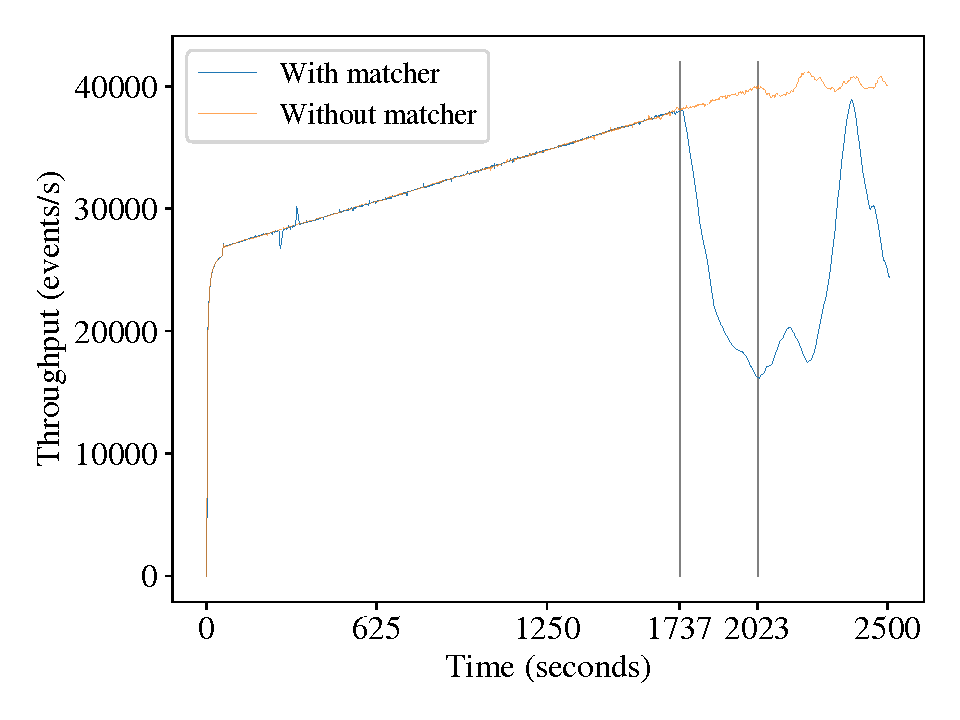
\includegraphics[width=1.0\textwidth]{figures/diffstream/throughput-accelerated.pdf}
        \caption{}\label{fig:throughput}
    \end{subfigure}%
    \begin{subfigure}[t]{0.33\textwidth}
        \centering
        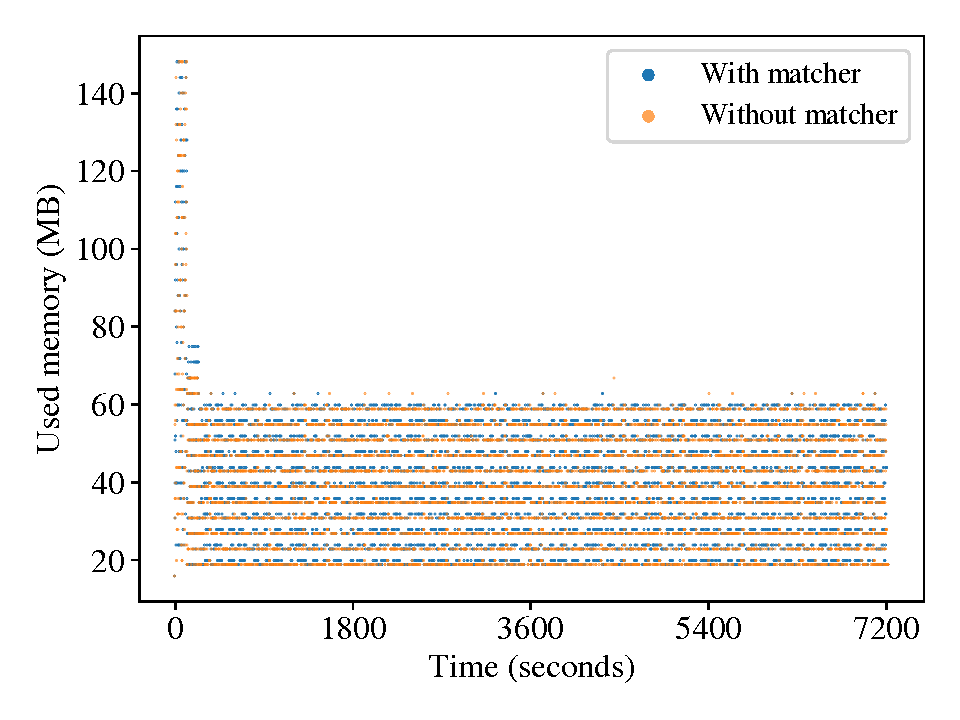
\includegraphics[width=1.0\textwidth]{figures/diffstream/used_memory_in_time.pdf}
        \caption{}\label{fig:memory-in-time}
    \end{subfigure}%
    \begin{subfigure}[t]{0.33\textwidth}
        \centering
        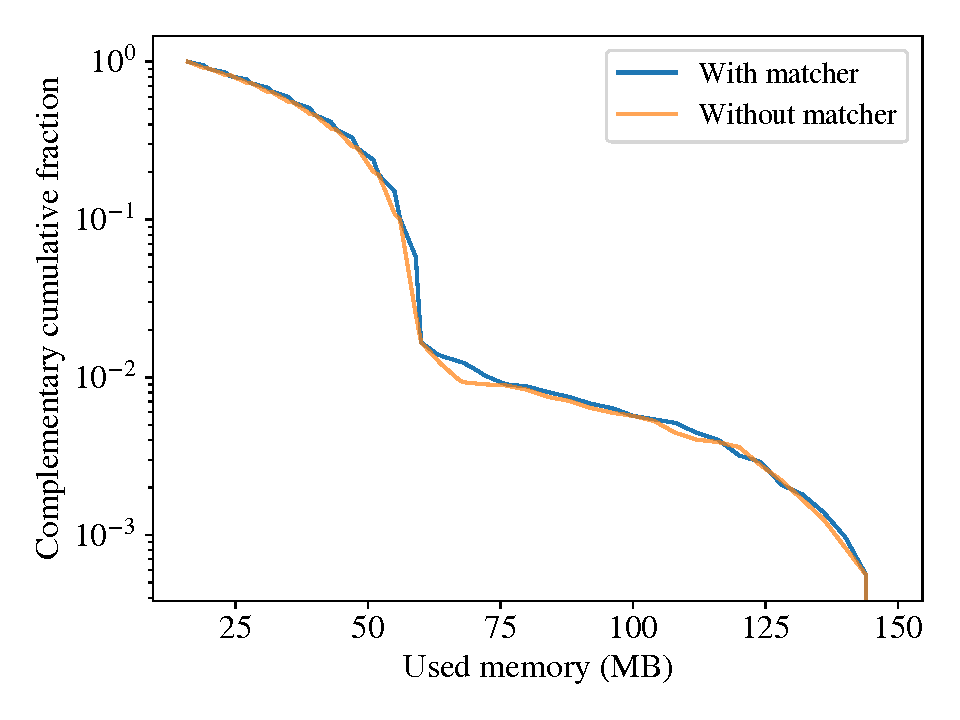
\includegraphics[width=1.0\textwidth]{figures/diffstream/memory_ccdf.pdf}
        \caption{}\label{fig:memory-ccdf}
    \end{subfigure}%
    \\
    \begin{subfigure}[t]{0.33\textwidth}
        \centering
        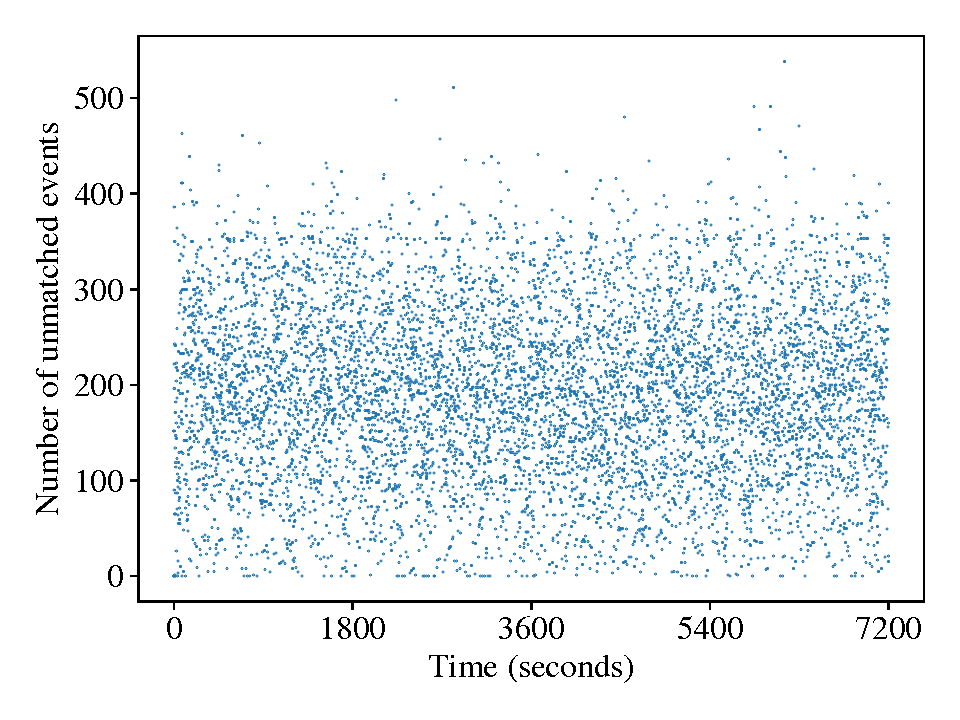
\includegraphics[width=1.0\textwidth]{figures/diffstream/unmatched_in_time.pdf}
        \caption{}\label{fig:unmatched-in-time}
    \end{subfigure}%
    \begin{subfigure}[t]{0.33\textwidth}
        \centering
        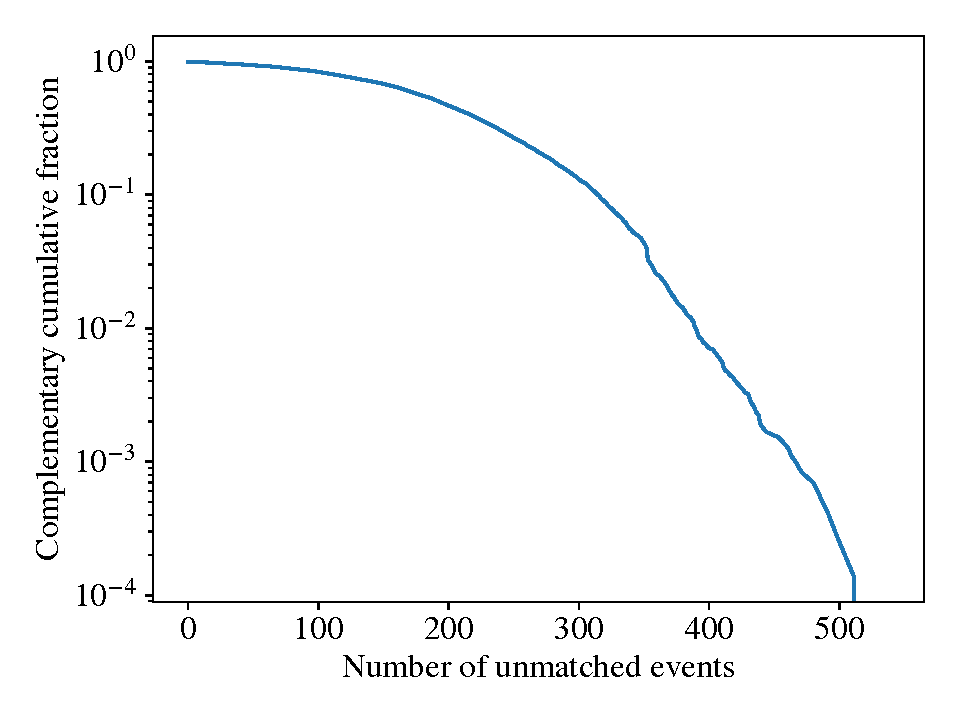
\includegraphics[width=1.0\textwidth]{figures/diffstream/unmatched_ccdf.pdf}
        \caption{}\label{fig:unmatched-ccdf}
    \end{subfigure}%
    \begin{subfigure}[t]{0.33\textwidth}
        \centering
        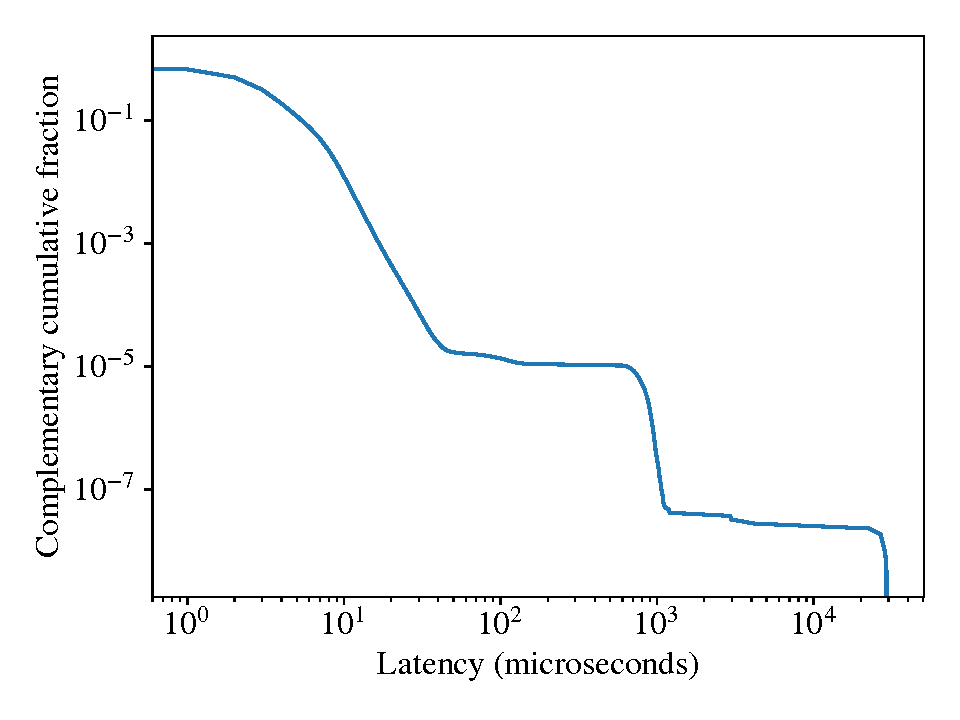
\includegraphics[width=1.0\textwidth]{figures/diffstream/latencies.pdf}
        \caption{}\label{fig:latencies}
    \end{subfigure}
    \caption{Results of the fourth case study: performance measurements of monitoring an application with DiffStream on the Yahoo streaming benchmark over a span of 2 hours, compared to the same application without the DiffStream matcher.}
\label{fig:online-perf-results}
\end{figure}
